\section{Trasformata Discreta di Fourier}
    Si definisce Trasformata Discreta di Fourier:
    \begin{gather}
        x_{[nT]} \overunderset{TDF}{ATDF}{\rightleftharpoons} \overline{X}_{(f)} \nonumber \\
        \overline{X}_{(f)} \in \mathbb{C}: \begin{cases}
            \left| \overline{X}_{(f)} \right| \nonumber \\
            \angle \overline{X}_{(f)} \nonumber
        \end{cases} \text{é una funzione periodica di periodo }\frac{1}{T}\nonumber  
    \end{gather}
    \subsubsection{Equazione di Analisi - $TDF$} \label{TDF}
        \[
            \overline{X}_{(f)} = \sum_{n=-\infty}^{\infty} x_{[nT]}e^{-j2\pi fnT}
        \]
    \subsubsection{Equazione di Sintesi - $ATDF$} \label{ATDF}
        \[
            x_{[nT]} = \frac{1}{2\pi} \int_{2\pi} \overline{X}_{(f)}e^{j2\pi fnT} df
        \]
    \subsubsection{Trasformata di $\delta_{[n]}$}\label{tdf sequenza di delta}
        \begin{gather}
            \sum_{n=-\infty}^{\infty}\delta_{(t-nT)} \overset{\ref{prima formula di poisson}}{=} \frac{1}{T} \sum_{k=-\infty}^{\infty} \Delta_{(\frac{k}{T})}e^{-j2\pi \frac{k}{T}t} \overset{\Delta \text{ costante}}{=} \frac{1}{T} \sum_{k=-\infty}^{\infty} e^{-j2\pi \frac{k}{T}t} \nonumber \\
            \Downarrow TCF\nonumber \\
            \sum_{n=-\infty}^{\infty}e^{-j2\pi fnT} = \frac{1}{T} \sum_{k=-\infty}^{\infty} \delta_{(f-\frac{k}{T})}\nonumber
        \end{gather}
        Applicando il ritardo:
        \[
            \sum_{n=-\infty}^{\infty}e^{-j2\pi (f-\nu)nT} = \frac{1}{T} \sum_{k=-\infty}^{\infty} \delta_{((f-\nu)-\frac{k}{T})}
        \]
    \subsubsection{Relazione tra $TCF$ e $TDF$}\label{Relazione tra $TCF$ e $TDF$}
        \begin{align}
            \overline{X}_{(f)} &= \sum_{n=-\infty}^{\infty} x_{[nT]}e^{-j2\pi fnT} = \sum_{n=-\infty}^{\infty} \underset{(\nu)}{\int_{-\infty}^{\infty}} X_{(\nu)} e^{-j2\pi \nu nT} d\nu e^{-j2\pi fnT} \nonumber \\
                               &= \underset{(\nu)}{\int_{-\infty}^{\infty}} X_{(\nu)} \sum_{n=-\infty}^{\infty} e^{-j2\pi \nu nT} e^{-j2\pi fnT} d\nu \overset{\ref{tdf sequenza di delta}}{=} \underset{(\nu)}{\int_{-\infty}^{\infty}} X_{(\nu)} \sum_{n=-\infty}^{\infty} \frac{1}{T} \delta_{((f-\nu)-\frac{k}{T})} d\nu  \nonumber \\
                               &\overset{\ref{Propietá del Delta di Dirac}:\text{paritá}}{=} \underset{(\nu)}{\int_{-\infty}^{\infty}} X_{(\nu)} \frac{1}{T} \sum_{n=-\infty}^{\infty}  \delta_{(\nu-(f-\frac{k}{T}))} d\nu = \frac{1}{T} \sum_{n=-\infty}^{\infty} \underset{(\nu)}{\int_{-\infty}^{\infty}} X_{(\nu)} \delta_{(\nu-(f-\frac{k}{T}))} d\nu  \nonumber \\
                               &\overset{\ref{Propietá del Delta di Dirac}:\text{campionatrice}}{=}  \frac{1}{T} \sum_{n=-\infty}^{\infty} X_{(f-\frac{k}{T})} \nonumber
        \end{align}
        quindi la $TDF$ si ottiene periodicizzando la $TCF$ con periodo $\frac{1}{T}$:
        \[
            \overline{X}_{(f)} = \frac{1}{T} \sum_{n=-\infty}^{\infty} X_{(f-\frac{k}{T})} 
        \] 
        \begin{figure}[H]
            \centering
            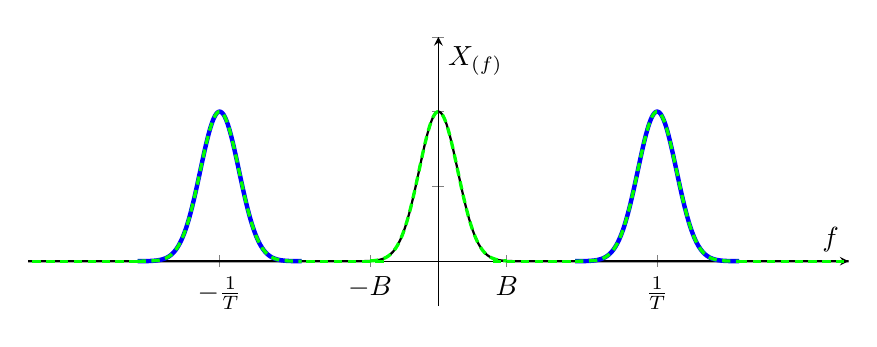
\begin{tikzpicture}
                \begin{axis}[
                    domain=-15:15,
                    samples=200,
                    axis lines=middle,
                    xlabel=$f$,
                    ylabel=$X_{(f)}$,
                    ymin=-0.3,
                    ymax=1.5,
                    xtick={-8,-2.5,2.5,8},
                    xticklabels={$-\frac{1}{T}$,$-B$,$B$,$\frac{1}{T}$},
                    ytick={},
                    yticklabels={},
                    width=12cm,
                    height=5cm
                ]

                \addplot [thick,black, samples = 800] {exp(-x^2)};
                \addplot [ultra thick,blue, domain = -11:-5, samples = 800] {exp(-(x+8)^2)};
                \addplot [ultra thick,blue, domain = 5:11, samples = 800] {exp(-(x-8)^2)};

                \addplot [densely dashed,very thick,green, domain = -2.5:2.5, samples = 900] {exp(-x^2)};
                \addplot [densely dashed,very thick,green, domain = -11:-5, samples = 800] {exp(-(x+8)^2)};
                \addplot [densely dashed,very thick,green, domain = 5:11, samples = 800] {exp(-(x-8)^2)};
                \addplot [densely dashed,very thick,green] coordinates{(-11,0)(-15,0)};
                \addplot [densely dashed,very thick,green] coordinates{(11,0)(15,0)};
                \addplot [densely dashed,very thick,green] coordinates{(-2,0)(-5,0)};
                \addplot [densely dashed,very thick,green] coordinates{(2,0)(5,0)};

                \end{axis}
            \end{tikzpicture}
            \caption{${\color{black} X_{(f)}}$,${\color{blue} X_{(f-\frac{k}{T})}}$,${\color{green} \overline{X}_{(f)}}$}
            \label{fig:relazione tdf tcf}
        \end{figure}
    \subsection{Teorema del Campionamento - Nyquist Shannon}\label{Teorema del Campionamento - Nyquist Shannon}
        \begin{figure}[H]
            \centering
                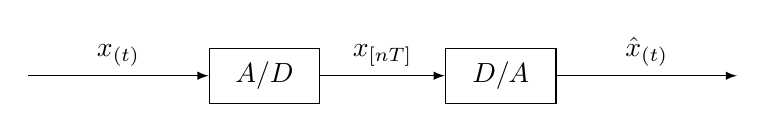
\begin{tikzpicture}[
                        node distance=3cm,
                        >=latex
                    ]
                    % Blocks
                    \node [coordinate] (input) {};
                    \node [rectangle, draw,minimum height=2em, minimum width=4em,right of=input] (AD) {$A/D$};
                    \node [rectangle, draw,minimum height=2em, minimum width=4em,right of=AD] (DA) {$D/A$};
                    \node [coordinate,right of=DA] (output) {};
                
                    % Connections
                    \draw [->] (input) --node[above]{$x_{(t)}$} (AD);
                    \draw [->] (AD) --node[above]{$x_{[nT]}$} (DA);
                    \draw [->] (DA) --node[above]{$\hat{x}_{(t)}$} (output);
                \end{tikzpicture}    
            \label{fig:Sistema di campionamento e ricostruzione}
            \caption{Esempio sistema campionamento e ricostruzione}
        \end{figure}
        \begin{itemize}
            \item {
                A/D: Campionatore, converte da analogico a discreto.
            }
            \item {
                A/D: interpolatore o filtro $p$, converte da discreto a analogico.
            }
        \end{itemize}
        Il nostro obbiettivo é dimensionare T e l'interpolatore in modo tale da poter ricostruire il segnale $\hat{x}:\ \hat{x} =x$.
        \paragraph{Dimensioniamo l'$A/D$:} Riprendiamo la relazione tra $TDF$ e $TCF$:
        \begin{figure}[H]
            \centering
            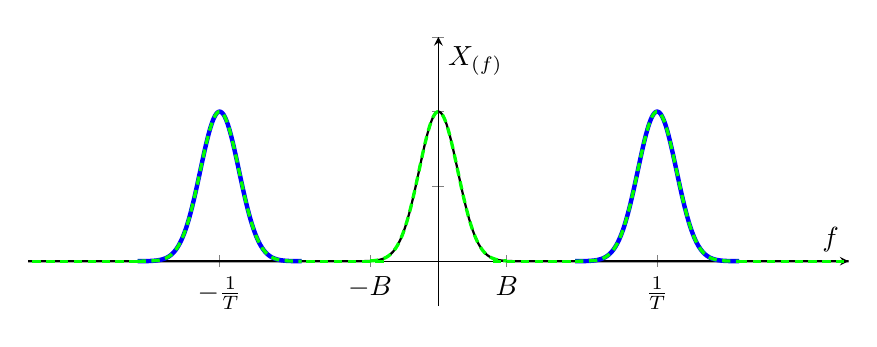
\begin{tikzpicture}
                \begin{axis}[
                    domain=-15:15,
                    samples=200,
                    axis lines=middle,
                    xlabel=$f$,
                    ylabel=$X_{(f)}$,
                    ymin=-0.3,
                    ymax=1.5,
                    xtick={-8,-2.5,2.5,8},
                    xticklabels={$-\frac{1}{T}$,$-B$,$B$,$\frac{1}{T}$},
                    ytick={},
                    yticklabels={},
                    width=12cm,
                    height=5cm
                ]
                
                \addplot [thick,black, samples = 800] {exp(-x^2)};
                \addplot [ultra thick,blue, domain = -11:-5, samples = 800] {exp(-(x+8)^2)};
                \addplot [ultra thick,blue, domain = 5:11, samples = 800] {exp(-(x-8)^2)};

                \addplot [densely dashed,very thick,green, domain = -2.5:2.5, samples = 900] {exp(-x^2)};
                \addplot [densely dashed,very thick,green, domain = -11:-5, samples = 800] {exp(-(x+8)^2)};
                \addplot [densely dashed,very thick,green, domain = 5:11, samples = 800] {exp(-(x-8)^2)};
                \addplot [densely dashed,very thick,green] coordinates{(-11,0)(-15,0)};
                \addplot [densely dashed,very thick,green] coordinates{(11,0)(15,0)};
                \addplot [densely dashed,very thick,green] coordinates{(-2,0)(-5,0)};
                \addplot [densely dashed,very thick,green] coordinates{(2,0)(5,0)};

                \end{axis}
            \end{tikzpicture}
            \caption{${\color{black} X_{(f)}}$,${\color{blue} X_{(f-\frac{k}{T})}}$,${\color{green} \overline{X}_{(f)} = \frac{1}{T}\sum_{k=-\infty}^{\infty}X_{(f-\frac{k}{T})}}$}
            \label{fig:relazione tdf tcf campionamento f 2B}
        \end{figure}

        abbiamo trovato che la $TDF$  non é altro che la periodicizzazione della $TCF$ con periodo $\frac{1}{T}$: se $\frac{1}{T}\geq 2B$
        il grafico ${\color{blue} X_{(f-\frac{k}{T})}}$ sono copie distinte non distorte e periodicizzate di $X_{(f)}$ da cui con un Filtro Passa-Basso \ref{Filtro Passa Basso di banda B - Low Pass Filter (LP)} 
        possiamo ricostruire il segnale. Se scegliessi $\frac{1}{T}<2B$:
        \begin{figure}[H]
            \centering
            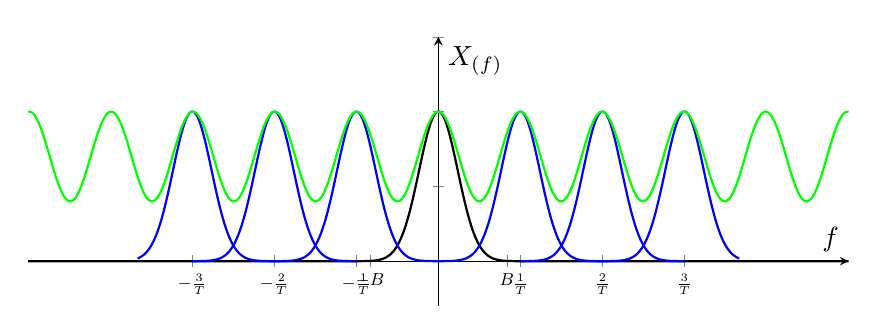
\begin{tikzpicture}
                \begin{axis}[
                    domain=-15:15,
                    samples=200,
                    axis lines=middle,
                    xlabel=$f$,
                    ylabel=$X_{(f)}$,
                    ymin=-0.3,
                    ymax=1.5,
                    xtick={-9,-6,-3,-2.5,2.5,3,9,6},
                    xticklabels={$-\frac{3}{T}$,$-\frac{2}{T}$,$-\frac{1}{T}$,$-B$,$B$,$\frac{1}{T}$,$\frac{3}{T}$,$\frac{2}{T}$,},
                    xticklabel style={font = \small,scale = 0.7},
                    ytick={},
                    yticklabels={},
                    width=12cm,
                    height=5cm
                ]
                
                \addplot [thick,black, samples = 800] {exp(-x^2)};
                \addplot [thick,blue, domain = -6:0, samples = 800] {exp(-(x+3)^2)};
                \addplot [thick,blue, domain = 0:6, samples = 800] {exp(-(x-3)^2)};

                \addplot [thick,blue, domain = -9:-3, samples = 800] {exp(-(x+6)^2)};
                \addplot [thick,blue, domain = 3:9, samples = 800] {exp(-(x-6)^2)};

                \addplot [thick,blue, domain = -11:-6, samples = 800] {exp(-(x+9)^2)};
                \addplot [thick,blue, domain = 6:11, samples = 800] {exp(-(x-9)^2)};

                \addplot [thick,green , samples = 800] {0.3*cos(deg(2.1*x))+0.7};

                \end{axis}
            \end{tikzpicture}
            \caption{${\color{black} X_{(f)}}$,${\color{blue} X_{(f-\frac{k}{T})}}$,${\color{green} \overline{X}_{(f)} = \frac{1}{T}\sum_{k=-\infty}^{\infty}X_{(f-\frac{k}{T})}}$}
            \label{fig:relazione tdf tcf campionamento f sbagliata}
        \end{figure}
        ho sovrapposizione delle copie di $X_{(f)}$ é il fenomeno di Aliasing: ho sovrapposizione di segnali che alterano il segnale originale. 
        In entrambi i casi ci troviamo in condizione di un segnale a banda limitata, nel tempo rappresenta un segnale illimitato.
        \paragraph{Dimensioniamo il $D/A$:}
        Partiamo dalla relazione di $\hat{x}$:
        \[
            \hat{x} = \sum_{n=-\infty}^{\infty}x_{[nT]}p_{(t-nT)},\ p\text{ interpolatore}
        \]
        Il segnale di uscita dal sistema dipende non solo dal periodo di campionamento $\frac{1}{T}$ ma anche dall'interpolatore che utilizziamo:
        \begin{itemize}
            \item {Interpolatore a mantenimento: mantiene il valore del segnale $x_{[nT]}$ per un periodo $T$
                \begin{figure}[H]
                    \centering
                    \begin{tikzpicture}
                        \begin{axis}[
                            domain=-5:5,
                            samples=200,
                            axis lines=middle,
                            xlabel=$t$,
                            ylabel=$p_{(t)}$,
                            ymin=-0.3,
                            ymax=5,
                            xmax=5,
                            xtick={3},
                            xticklabels={$T$},
                            ytick={1.5},
                            width=9cm,
                            height=4.5cm
                        ]
                        %x(t)
                        \addplot [const plot, thick, orange] coordinates{(0,0)(0,1.5)(3,1.5)(3,0)};
                        %Colors
                        \end{axis}
                    \end{tikzpicture}
                    \caption{Interpolatore a mantenimento}
                    \label{fig:interpolatore a mantenimento}
                \end{figure}
                \begin{figure}[H]
                    \centering
                    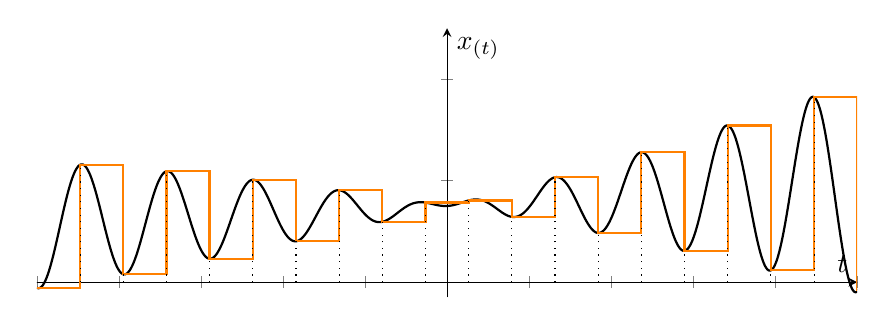
\begin{tikzpicture}
                        \begin{axis}[
                            domain=-5:5,
                            samples=200,
                            axis lines=middle,
                            xlabel=$t$,
                            ylabel=$x_{(t)}$,
                            ymin=-0.3,
                            ymax=5,
                            xtick={},
                            xticklabels={},
                            ytick={},
                            yticklabels={},
                            width=12cm,
                            height=5cm
                        ]
                        %x(t)
                        \addplot [thick,black, samples = 1000] {(x/3*sin(deg(6*x))+1.5)*((x/20)+1)};
                        \addplot [const plot,thick,orange, samples = 20] {(x/3*sin(deg(6*x))+1.5)*((x/20)+1)};
                        \addplot+ [ycomb, mark = none, dotted, black, samples = 20] {(x/3*sin(deg(6*x))+1.5)*((x/20)+1)};
                        %Colors
                        \end{axis}
                    \end{tikzpicture}
                    \caption{$x_{(t)}$,{\color{orange}$\hat{x} = \sum_{n=-\infty}^{\infty}x_{[nT]}p_{(t-nT)}$}}
                    \label{fig:x con interpolatore a mantenimento}
                \end{figure}
            }
            \item {Interpolatore Lineare: incrementa linearmente il valore di $\hat{x}$
                \begin{figure}[H]
                    \centering
                    \begin{tikzpicture}
                        \begin{axis}[
                            domain=-5:5,
                            samples=200,
                            axis lines=middle,
                            xlabel=$t$,
                            ylabel=$p_{(t)}$,
                            ymin=0.3,
                            xmin=-5,
                            ymax=5,
                            xmax=5,
                            xtick={-1.7,1.7},
                            xticklabels={$-\frac{T}{2}$,$\frac{T}{2}$},
                            ytick={2},
                            yticklabels={$1$},
                            width=9cm,
                            height=5cm
                        ]
                        \addplot [sharp plot,thick,orange] coordinates{(-2,0)(0,2)(2,0)};
                        \end{axis}
                    \end{tikzpicture}
                    \caption{Interpolatore Lineare}
                    \label{fig:interpolatore Lineare}
                \end{figure}
                \begin{figure}[H]
                    \centering
                    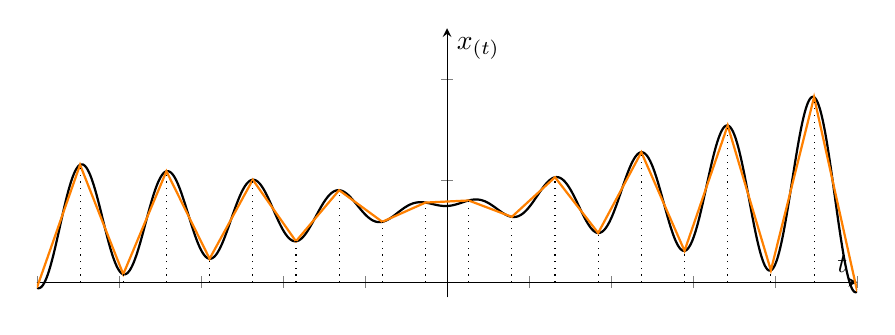
\begin{tikzpicture}
                        \begin{axis}[
                            domain=-5:5,
                            samples=200,
                            axis lines=middle,
                            xlabel=$t$,
                            ylabel=$x_{(t)}$,
                            ymin=-0.3,
                            ymax=5,
                            xtick={},
                            xticklabels={},
                            ytick={},
                            yticklabels={},
                            width=12cm,
                            height=5cm
                        ]
                        
                        \addplot [thick,black, samples = 1000] {(x/3*sin(deg(6*x))+1.5)*((x/20)+1)};
                        \addplot [sharp plot,thick,orange, samples = 20] {(x/3*sin(deg(6*x))+1.5)*((x/20)+1)};
                        \addplot+ [ycomb, mark = none, dotted, black, samples = 20] {(x/3*sin(deg(6*x))+1.5)*((x/20)+1)};
                        \end{axis}
                    \end{tikzpicture}
                    \caption{$x_{(t)}$,{\color{orange}$\hat{x} = \sum_{n=-\infty}^{\infty}x_{[nT]}p_{(t-nT)}$}}
                    \label{fig:x con interpolatore Lineare}
                \end{figure}
            }
        \end{itemize}
        Passiamo alla frequenza:
        \[
            \hat{x} = \sum_{n=-\infty}^{\infty}x_{[nT]}p_{(t-nT)} \overset{TCF}{\rightleftharpoons} \hat{X}_{(f)} = \sum_{n=-\infty}^{\infty}x_{[nT]}P_{(f)}e^{-j2\pi fnT}
        \]
        \begin{gather}
            \hat{X}_{(f)} = P_{(f)}\sum_{n=-\infty}^{\infty}x_{[nT]}e^{-j2\pi fnT} = P_{(f)}\overline{X}_{(f)} \nonumber \\
            Se\ \hat{x}=x\ anche\ \hat{X}_{(f)} = X_{(f)}\nonumber \\
            \Downarrow \ref{Relazione tra $TCF$ e $TDF$} \nonumber \\
            X_{(f)} \overset{!}{=} P_{(f)}\frac{1}{T}\sum_{k=-\infty}^{\infty}X_{(f-\frac{k}{T})} \nonumber
        \end{gather}
        dobbiamo dimensionare $P_{(f)}$ in modo tale da rendere vera $\hat{X}_{(f)} = X_{(f)}$
        \begin{figure}[H]
            \centering
            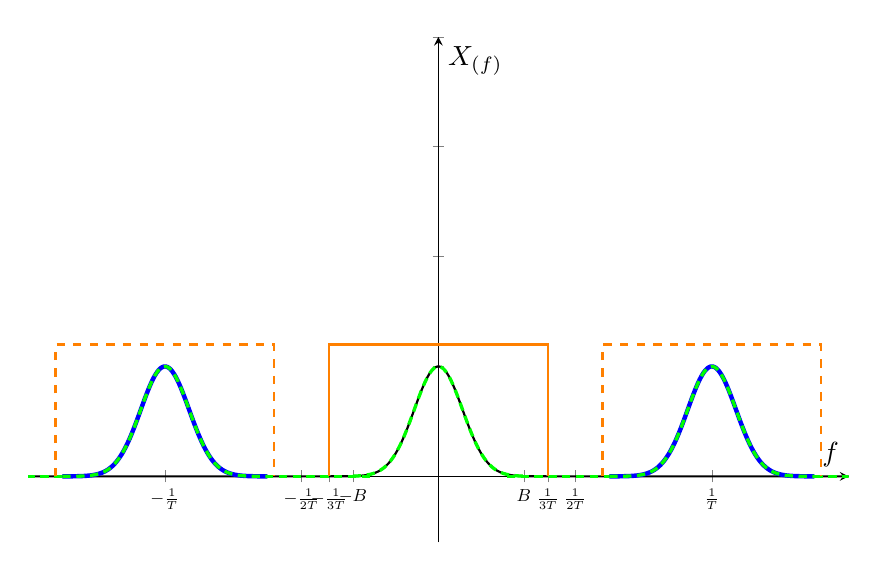
\begin{tikzpicture}
                \begin{axis}[
                    domain=-12:12,
                    samples=200,
                    axis lines=middle,
                    xlabel=$f$,
                    ylabel=$X_{(f)}$,
                    ymin=-0.3,
                    ymax=2,
                    xmax=12,
                    xmin=-12,
                    xtick={-8,-4,-3.2,-2.5,2.5,3.2,4,8},
                    xticklabels={$-\frac{1}{T}$,$-\frac{1}{2T}$,$-\frac{1}{3T}$,$-B$,$B$,$\frac{1}{3T}$,$\frac{1}{2T}$,$\frac{1}{T}$},
                    xticklabel style={font = \small,scale = 0.7},
                    ytick={},
                    yticklabels={},
                    width=12cm,
                    height=8cm 
                ]
                
                \addplot [thick,black, samples = 800] {0.5*exp(-x^2)};
                \addplot [ultra thick,blue, domain = -11:-5, samples = 800] {0.5*exp(-(x+8)^2)};
                \addplot [ultra thick,blue, domain = 5:11, samples = 800] {0.5*exp(-(x-8)^2)};

                \addplot [densely dashed,very thick,green, domain = -2.5:2.5, samples = 900] {0.5*exp(-x^2)};
                \addplot [densely dashed,very thick,green, domain = -11:-5, samples = 800] {0.5*exp(-(x+8)^2)};
                \addplot [densely dashed,very thick,green, domain = 5:11, samples = 800] {0.5*exp(-(x-8)^2)};
                
                \addplot [densely dashed,very thick,green] coordinates{(-11,0)(-15,0)};
                \addplot [densely dashed,very thick,green] coordinates{(11,0)(15,0)};
                \addplot [densely dashed,very thick,green] coordinates{(-2,0)(-5,0)};
                \addplot [densely dashed,very thick,green] coordinates{(2,0)(5,0)};

                \addplot [const plot, thick,orange] coordinates{(-3.2,0)(-3.2,0.6)(3.2,0.6)(3.2,0)};
                \addplot [const plot, dashed ,thick,orange] coordinates{(-11.2,0)(-11.2,0.6)(-4.8,0.6)(-4.8,0)};
                \addplot [const plot, dashed ,thick,orange] coordinates{(4.8,0)(4.8,0.6)(11.2,0.6)(11.2,0)};

                \end{axis}
            \end{tikzpicture}
            \caption{${\color{black} X_{(f)}}$,${\color{blue} X_{(f-\frac{k}{T})}}$,${\color{orange} P_{(f)}}$}
            \label{fig:tdf tcf dimansionamento interpolatore}
        \end{figure}
        Utilizziamo un filtro passa basso che abbia una durata in banda maggiore di $2B$ ma minore di $\frac{1}{2T}$  per lasciarci un pochino di margine e evitare  di prendere 
        la copia del segnale successivo/precedente ($2B<T_r\leq\frac{1}{2T_s}$): prendiamo una durata $\frac{1}{2T_s}>2B$
        \[
            P_{(f)} = T rect\left(\frac{f}{2\frac{1}{2T}}\right)= T rect\left(fT\right) \overset{TCF}{\leftrightharpoons} p_{(t)} = \frac{T}{T}sinc\left(\frac{t}{T}\right)
        \]
        
        \paragraph{Interpolatore a seno cardinale:} Si utilizza un interpolatore a seno cardinale
            \begin{figure}[H] $he$
                \centering
                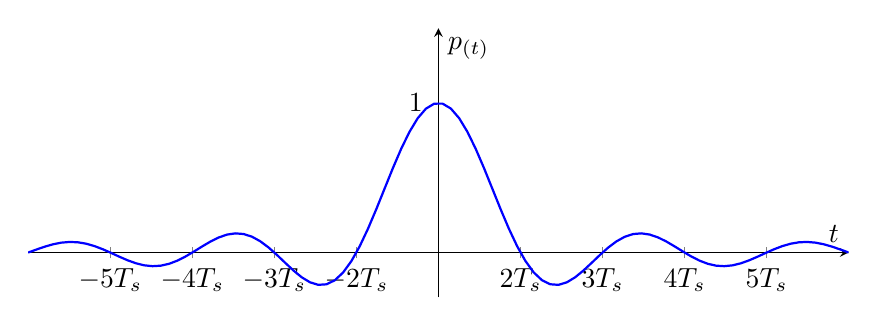
\begin{tikzpicture}
                    \begin{axis}[
                        domain=-5:5,
                        samples=200,
                        axis lines=middle,
                        xlabel=$t$,
                        ylabel=$p_{(t)}$,
                        ymin=-0.3,
                        ymax=1.5,
                        xtick={-4,-3,-2,-1,-0,0,0,1,2,3,4},
                        xticklabels={$-5T_s$,$-4T_s$,$-3T_s$,$-2T_s$,$-T_s$,$0$,$T_s$,$2T_s$,$3T_s$,$4T_s$,$5T_s$},
                        ytick={1},
                        yticklabels={$1$},
                        width=12cm,
                        height=5cm
                    ]
                    %x(t)
                    \addplot [blue, thick, samples = 100] {sin(deg(x*pi))/(x*pi)};
                    \end{axis}
                \end{tikzpicture}
                \caption{Interpolatore a seno cardinale}
                \label{fig:interpolatore a seno cardinale}
            \end{figure}
            \begin{figure}[H]
                \centering
                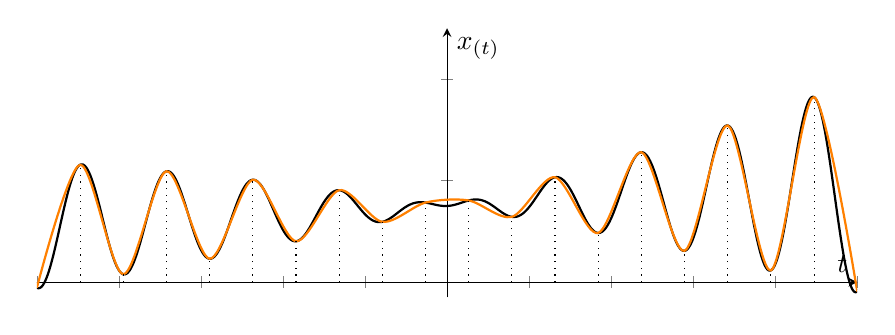
\begin{tikzpicture}
                    \begin{axis}[
                        domain=-5:5,
                        samples=200,
                        axis lines=middle,
                        xlabel=$t$,
                        ylabel=$x_{(t)}$,
                        ymin=-0.3,
                        ymax=5,
                        xtick={},
                        xticklabels={},
                        ytick={},
                        yticklabels={},
                        width=12cm,
                        height=5cm
                    ]
                    \addplot [thick,black, samples = 1000] {(x/3*sin(deg(6*x))+1.5)*((x/20)+1)};
                    \addplot [smooth,thick,orange, samples = 20] {(x/3*sin(deg(6*x))+1.5)*((x/20)+1)};
                    \addplot+ [ycomb, mark = none, dotted, black, samples = 20] {(x/3*sin(deg(6*x))+1.5)*((x/20)+1)};

                    \end{axis}
                \end{tikzpicture}
                \caption{$x_{(t)}$,{\color{orange}$\hat{x} = \sum_{n=-\infty}^{\infty}x_{[nT]}p_{(t-nT)}$}}
                \label{fig:x con interpolatore a seno cardinale}
            \end{figure}
            l'interpolatore a seno cardinale non é causale: essendo delle $sinc$ a ogni campionamento, non posso conoscere il peso delle $sinc$ 
            dei valori della sequenza successivi. Se opero non Real Time (Virtuale), invece ho infiniti campioni a cui posso attingere: Risolvo entrambi i 
            problemi troncando la $sinc$ e spostandola a dx, ma per troncarla sto moltiplicando una $sinc$ per una $rect$ nel tempo, passando alla frequenza 
            la funzione limitata nel tempo diventa illimitata in frequenza andando a influenzare anche le repliche successive.


        
        \paragraph{Teorema del Campionamento:} Dato un segnale analogico $x_{(t)}$ la cui banda di frequenze sia limitata e dato $c\in \mathbb{Z}$,
        il segnale $x_{(t)}$ puó essere univocamente ricostruito a partire dai suoi campioni $x_{[nT]}$ presi a frequenza (o periodo) $f_s = \frac{1}{T}$ se 
        $f_s = \frac{1}{T} \geq 2B$ mediante:
        \[
            x_{(t)} = \sum_{n=-\infty}^{\infty} x_{[nT]}sinc\left(\frac{t}{T}-n\right) 
        \]
        Criticitá
        \begin{itemize}
            \item {Segnale a banda limitata}
            \item {Interpolatore dimensionato}
        \end{itemize}
        Osservazioni: Se utilizzassi un filtro con durata $\frac{1}{T}>>2B$ prenderei tantissimi campioni che
        non servono per ricostruire meglio il segnale: dagli esempi di matlab possiamo vedere che ci basta anche solo un periodo uguale a $2B$.\\
        Esempio:
        \[
            B = 10KHz,\ 2B = 20KHz,\ \text{Durata filtro} = 25KHz\ ho\ 5KHz\text{ di margine}
        \]
        Esempio:$f_s = \frac{1}{T} = 2B,\ p_{(t)}=sinc(2Bt)$
        \begin{gather}
                \hat{x}_{(t)} = \sum_{n=-\infty}^{\infty} x_{[nT]}sinc\left(2Bt_0 -n\right) \nonumber \\
                \hat{x}_{(t_0)} = \sum_{n=-\infty}^{\infty} x_{[nT]}sinc\left(2Bt_0 -n\right) \nonumber
        \end{gather}
        $\hat{x}_{(t_0)}$ dipende dal contributo di tutte le $sinc$ anche dei valori successivi, per questo si pone il problema del filtro causale. 
        \begin{figure}[H]
            \centering
            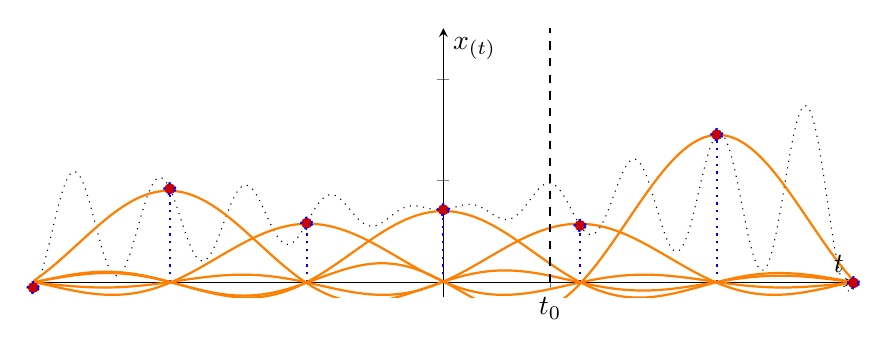
\begin{tikzpicture}
                \begin{axis}[
                    domain=-5:5,
                    samples=200,
                    axis lines=middle,
                    xlabel=$t$,
                    ylabel=$x_{(t)}$,
                    ymin=-0.3,
                    ymax=5,
                    xtick={1.3},
                    xticklabels={$t_0$},
                    ytick={},
                    yticklabels={},
                    width=12cm,
                    height=5cm
                ]
                % 0.53 periodo
                \addplot [thin,dotted,black, samples = 1000] {(x/3*sin(deg(6*(x-1)))+1.5)*(((x-1)/20)+1)};
                \addplot+ [ycomb, mark = *, dotted, blue,thick, samples = 7] {(x/3*sin(deg(6*(x-1)))+1.5)*(((x-1)/20)+1)};
                % Sinc x positive
                \addplot [orange, thick, samples = 500] {1.4*sin(deg((x)*pi*0.6))/((x)*pi*0.6)};
                \addplot [orange, thick, samples = 500] {1.15*sin(deg((x-1.65)*pi*0.6))/((x-1.65)*pi*0.6)};
                \addplot [orange, thick, samples = 500] {2.9*sin(deg((x-3.35)*pi*0.6))/((x-3.35)*pi*0.6)};
                % \addplot [orange, thick, samples = 500] {1.3*sin(deg((x-1.325)*pi*2))/((x-1.325)*pi*2)};
                % \addplot [orange, thick, samples = 500] {1.3*sin(deg((x-1.855)*pi*2))/((x-1.855)*pi*2)};
                % \addplot [orange, thick, samples = 500] {1.3*sin(deg((x-2.385)*pi*2))/((x-2.385)*pi*2)};
                % \addplot [orange, thick, samples = 500] {1.3*sin(deg((x-2.915)*pi*2))/((x-2.915)*pi*2)};
                % \addplot [orange, thick, samples = 500] {1.3*sin(deg((x-3.445)*pi*2))/((x-3.445)*pi*2)};
                % \addplot [orange, thick, samples = 500] {1.3*sin(deg((x-3.975)*pi*2))/((x-3.975)*pi*2)};
                % \addplot [orange, thick, samples = 500] {1.3*sin(deg((x-4.505)*pi*2))/((x-4.505)*pi*2)};
                % Sinc x negative
                \addplot [orange, thick, samples = 500] {1.15*sin(deg((x+1.65)*pi*0.6))/((x+1.65)*pi*0.6)};
                \addplot [orange, thick, samples = 500] {1.8*sin(deg((x+3.35)*pi*0.6))/((x+3.35)*pi*0.6)};
                % \addplot [orange, thick, samples = 500] {1.3*sin(deg((x+1.855)*pi*2))/((x+1.855)*pi*2)};
                % \addplot [orange, thick, samples = 500] {1.3*sin(deg((x+2.385)*pi*2))/((x+2.385)*pi*2)};
                % \addplot [orange, thick, samples = 500] {1.3*sin(deg((x+2.915)*pi*2))/((x+2.915)*pi*2)};
                % \addplot [orange, thick, samples = 500] {1.3*sin(deg((x+3.445)*pi*2))/((x+3.445)*pi*2)};
                % \addplot [orange, thick, samples = 500] {1.3*sin(deg((x+3.975)*pi*2))/((x+3.975)*pi*2)};
                % \addplot [orange, thick, samples = 500] {1.3*sin(deg((x+4.505)*pi*2))/((x+4.505)*pi*2)};
                \addplot [black, thick,dashed] coordinates{(1.3,0)(1.3,5)};
                \end{axis}
            \end{tikzpicture}
            \caption{$x_{(t)}$,{\color{orange}$\hat{x} = \sum_{n=-\infty}^{\infty}x_{[nT]}p_{(t-nT)}$}}
            \label{fig:Interpolatore seno cardinale}
        \end{figure}
        I passi in un sistema A/D/A sono:
        \begin{itemize}
            \item {Passo dal tempo in frequenza: $x_{(t)} \overset{TCF}{\rightleftharpoons} X_{(f)}$}.
            \item {Osservo la banda che occupa il segnale e scelgo $B$.}
            \item {Scelgo una frequenza (periodo) di campionamento $f_s$ e calcolo $x_{[nT]}$.}
            \item {Calcolo $\hat{x}$ con un interpolatore a seno cardinale,$sinc$}
        \end{itemize}
























